\xiti
\begin{xiaotis}

\xiaoti{求证:球的任意两个大圆互相平分。}

\xiaoti{在半径是 13 cm 的球面上有 $A$、$B$、$C$ 三点, $AB = 6$ cm,
    $BC = 8$ cm, $CA = 10$ cm。 求经过这三点的截面和球心 $O$ 的距离。
}

\xiaoti{在半径是 $r$ 的球面上有两点 $A$、$B$,半径 $OA$ 和 $OB$ 的夹
    角是 $n^\circ \; (n < 180)$。求$A$、$B$ 两点间的球面距离。
}

\xiaoti{在北纬 $30^\circ$ 圈上有甲、乙两地,它们的经度相差 $120^\circ$,计算这两地间的纬度线长。}

\xiaoti{在赤道上,东经 $140^\circ$ 与西经 $130^\circ$ 的海面上有两点 $A$、$B$。
    求$A$、$B$ 两点的球面距离是多少海里?
}

\xiaoti{已知球的大圆的周长是 80 cm。 求这个球的表面积。}

\xiaoti{在球心的同一侧有相距 9 cm 的两个平行截面,它们的面积各为 $49\pi \; \pflm$
    和 $400\pi \; \pflm$。 求球的表面积。
}

\xiaoti{水箱用的胶质浮球,是由两个半球面和一个圆柱筒贴合而成。 已知球的半径是 3 cm,
    圆柱筒长 2 cm。 要在这样 2500 个浮球上涂一层胶质。如果每平方米需要涂胶 100 g,
    共需胶多少?
}

\xiaoti{半径是 4 cm 的球面,被一个平面截得的截面半径是 2 cm,求所截得的球冠的面积。}

\xiaoti{我国第一颗人造地球卫星的远地点距地面 2384 km,在这时约有多少平方公里上的人能看到这颗卫星?}

\begin{figure}[htbp]
    \centering
    \begin{minipage}[b]{7cm}
        \centering
        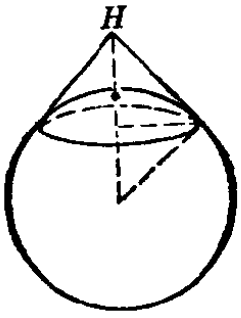
\includegraphics[width=3.5cm]{../pic/ltjh-ch2-xiti11-10.png}
        \caption*{(第 10 题)}
    \end{minipage}
    \qquad
    \begin{minipage}[b]{7cm}
        \centering
        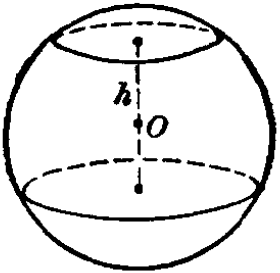
\includegraphics[width=4cm]{../pic/ltjh-ch2-xiti11-12.png}
        \caption*{(第 12 题)}
    \end{minipage}
\end{figure}

\xiaoti{有直径为 10 cm 的球,以它的一条直径为轴,钻一个直径为 6 cm 的圆孔,
    求这个球的球面剩余部分的面积。
}

\xiaoti{球面夹在两个平行截面间的部分叫做\zhongdian{球带},两个平行截面间的距离叫做\zhongdian{球带的高}。
    如果球的半径是 $R$,球带的高是 $h$,求证:\zhongdian{$\bm{S_\text{球带} = 2\pi Rh$}}。
}

\xiaoti{利用上题结果,计算地球上热带的面积。}

\end{xiaotis}

